\documentclass[11pt,a4paper,titlepage]{article}
\usepackage[utf8x]{inputenc}
\usepackage{ucs}
\usepackage{ulem}
\usepackage{amsmath}
\usepackage{amsfonts}
\usepackage{amssymb}
\usepackage{pdfpages}
\usepackage[linkbordercolor={1 1 1}, urlbordercolor={1 1 1}]{hyperref}
\usepackage[german]{babel}
\usepackage{eurosym}
\usepackage{pdfpages}
\usepackage{graphicx}
\usepackage{float}
\setcounter{secnumdepth}{4} 
\setlength{\parindent}{3em}
\usepackage[paper=a4paper,left=15mm,right=15mm,top=20mm,bottom=20mm]{geometry}
\pagestyle{plain} 
\title{{\Huge Benutzerhandbuch} \linebreak \linebreak

\includegraphics[width= 35px]{BilderHandbuch/icon32.png} \\
\textbf{Testsuite-Management}
\linebreak \linebreak Handbuch für die Version 1.5.2}
\usepackage[space,extendedchars]{grffile}
\begin{document}

\maketitle
\pagebreak

\tableofcontents
\pagebreak

\section{Vorwort}
Wir freuen uns, dass Sie sich für Testsuite-Management (TSM) entschieden haben.\\
TSM wurde im Rahmen eines Studienprojekts von Studenten der Universität Stuttgart im Bachelor-Studiengang Softwaretechnik entwickelt.

\section{Einleitung}
Dieses Handbuch ermöglicht Ihnen den Einstieg in die Verwendung des Eclipse-Plugins TSM und der alleinstehenden Programmversion in der Version 1.5.2.
Es erklärt Ihnen die Installation und die Benutzung.\\


\subsection{Lizenzbedingungen}
TSM steht unter der Eclipse Public License in der Version 1.0, die Sie unter \href{http://www.eclipse.org/legal/epl-v10.html}{http://www.eclipse.org/legal/epl-v10.html} finden können.

\subsection{Konventionen}
Benutzerelemente und Oberflächenelemente die ausgewählt werden, sind in \texttt{Schreibmaschinenschrift} dargestellt.

\section{Installation}
Das Programm wird in zwei Versionen ausgeliefert. Einmal als installierbare Eclipse-Update-Site und einmal als RCP-Produkt. \\


\subsection{Verwendung des RCP-Produkts}

\subsubsection{Voraussetzungen}
Sie benötigen:
\begin{enumerate}
 \item Java Runtime Environment in der Version 1.6 (Minimalvoraussetzung).
\end{enumerate}

\subsubsection{Installationsschritte}
\begin{enumerate}
 \item Entpacken Sie die "`tsmProduct-v1.5.1.2.zip"'-Datei.
 \item Führen Sie die ausführbare eclipse-Datei aus.
\end{enumerate}


\subsection{Installation der Eclipse-Update-Site}
TSM ist für Eclipse-RCP entwickelt und kann über den internen Plugin-Assistenten installiert werden.


\subsubsection{Voraussetzungen}
Sie benötigen für die Installation der Update-Site:
\begin{itemize}
 \item Java Runtime Environment in der Version 1.6 (Minimalvoraussetzung)\footnote{\href{http://www.oracle.com/technetwork/java/javase/downloads/index.html}
 {http://www.oracle.com/technetwork/java/javase/downloads/index.html}}
 \item Eclipse in der Version 4.2 (Minimalvoraussetzung)\footnote{\href{http://www.eclipse.org/downloads/packages/eclipse-ide-java-developers/junosr1}
 {http://www.eclipse.org/downloads/packages/eclipse-ide-java-developers/junosr1}}
 \item Die installierbare Plugin-Version von TSM.
\end{itemize}

\subsubsection{Installationsschritte}

\begin{enumerate}
 \item Starten Sie Eclipse und legen Sie einen neuen Workspace an.
 \item Klicken Sie in Eclipse auf \textit{Help}, \textit{Install New Software...}
 \item Klicken Sie im sich öffnenden Dialog auf \textit{Add...}.
 \item Klicken sie auf \textit{Archive...}
 \item Wählen Sie die "`tsmUpdateSite-v1.5.2.zip"'.
 \item Selektieren Sie \textit{TSM} und dann \textit{tsmFeature}.
 \item Stellen Sie sicher, dass die Option \textit{Contact all update sites during install to find required software} deaktiviert ist.
 \item Klicken Sie auf \textit{Next} und folgen Sie den Anweisungen des Assistenten.
 \item Nach dem Eclipse-Neustart können Sie mittels \textit{Window}, \textit{Open Perspective}, \textit{Other...} die TSM-Perspektive öffnen.
\end{enumerate}

\subsubsection{Fehlermeldung}
Wir bitten Sie, uns Fehler, die Sie finden mittels des Bug-Tracking-Werkzeuges Sourceforges unter \\ \href{https://sourceforge.net/p/tsmtest/tickets/}
{https://sourceforge.net/p/tsmtest/tickets/} mitzuteilen.

\section{Benutzung des TSM-Navigators}
In diesem Kapitel wird Ihnen die Benutzung von TSM mit dem TSM-Navigator erklärt. Der TSM-Navigator wurde speziell für TSM entwickelt.
Er befindet sich auf der linken Seite und zeigt alle Projekte und Testfälle. Im TSM-Navigator gibt es einen unsichtbaren Ordner \texttt{Images}. In diesem liegen die Bilder der Testfälle.
Dieser erscheint in manchen Assistenten, kann aber nicht ausgewählt werden. \textbf{In ihm dürfen keine Testfälle erstellt werden!}

\subsection{Projekt}
Ein Projekt ist der Überbegriff für eine Sammlung von Paketen und Testfällen.

\subsubsection{Projekt anlegen}
\begin{enumerate}
\item Klicken Sie im TSM-Navigator oben auf das Projekt-Symbol.
\begin{figure}[H]
\centering
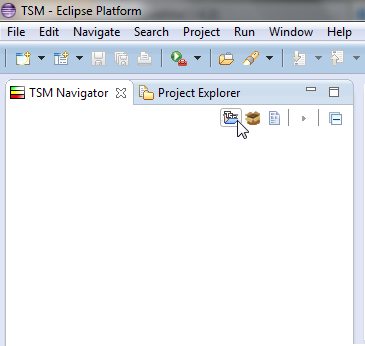
\includegraphics[width= 260px]{BilderHandbuchTSMNavigator/Projekt/Projekt.png}
\caption{TSM-Projekt anlegen}
\label{fig:Projekt}
\end{figure}
\item Es öffnet sich ein Assistent.

\begin{figure}[H]
\centering
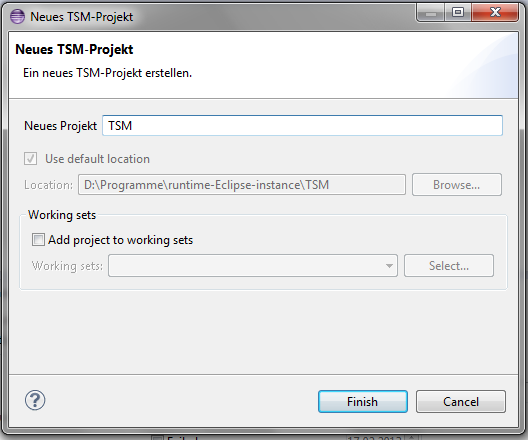
\includegraphics[width= 260px]{BilderHandbuchTSMNavigator/Projekt/ProjektAssistent.png}
\caption{TSM-Projekt-Assistent}
\label{fig:Projekt}
\end{figure}

\item Geben Sie im Assistenten in \texttt{Neues Projekt:} den Namen Ihres Projekts an und klicken auf \texttt{Finish}. Das Projekt liegt nun im TSM-Navigator.
\end{enumerate}
\textit{\textbf{Alternativ} können Sie auch per Rechtsklick im TSM-Navigator unter \texttt{New...} - \texttt{TSM-Projekt} ein Projekt anlegen.
Oder Sie öffnen per Tastenkombination \texttt{STRG+N} den Assistenten. Wählen Sie dort \texttt{TSM} und dann \texttt{TSM-Projekt} folgen Sie dem Assistenten.}

\subsubsection{Projekt umbenennen}
\begin{enumerate}
\item Machen Sie einen Rechtsklick auf das Projekt, das Sie umbenennen möchten und  klicken Sie auf \texttt{Umbenennen}.

\begin{figure}[H]
\centering
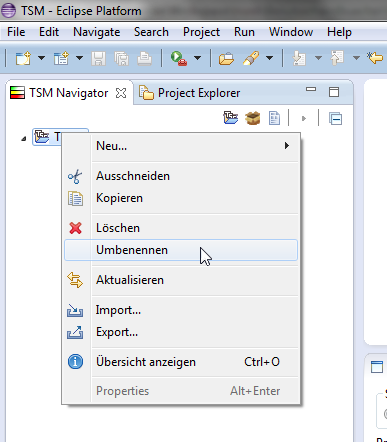
\includegraphics[width= 200px]{BilderHandbuchTSMNavigator/Projekt/ProjektUmbenennen.png}
\caption{Projekt umbenennen}
\label{fig:ProjektUmbenennen}
\end{figure}

\item Geben Sie nun den neuen Namen Ihres Projekts an und bestätigen Sie mit \texttt{Enter}. Bitte beachten Sie, dass die folgenden Zeichen nicht erlaubt sind: $ < > ? " : | _ . \setminus / *$
\end{enumerate}

\subsection{Paket}
Ein Paket ist eine Struktureinheit, um ein Projekt logisch untergliedern zu können. Pakete können Testfälle und weitere Pakete enthalten.

\subsubsection{Paket anlegen}
Um ein Paket anlegen zu können, muss bereits ein Projekt angelegt sein.
\linebreak

\begin{enumerate}
\item Selektieren Sie das Projekt oder Paket, in dem das neue Paket erstellt werden soll. Klicken Sie anschließend im TSM-Navigator auf das Paket-Symbol.

\begin{figure}[H]
\centering
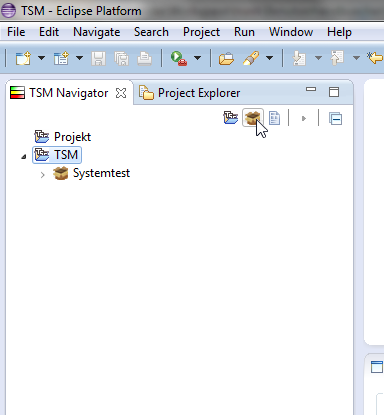
\includegraphics[width= 260px]{BilderHandbuchTSMNavigator/Paket/Paket.png}
\caption{Paket anlegen}
\label{fig:Paket}
\end{figure}
\end{enumerate}

\textit{\textbf{Alternativ} können Sie auch per Rechtsklick im TSM-Navigator unter \texttt{New...} - \texttt{TSM-Paket} ein Paket anlegen.
Oder per Tastenkombination \texttt{STRG+N} öffnet sich ein Assistent indem Sie unter dem Ordner \texttt{TSM} auf \texttt{TSM-Paket} klicken und dem Assistenten folgen.}

\subsubsection{Paket umbenennen}
\begin{enumerate}
\item Machen Sie einen Rechtsklick auf das Paket, das Sie umbenennen möchten und  klicken Sie auf \texttt{Umbenennen}.

\begin{figure}[H]
\centering
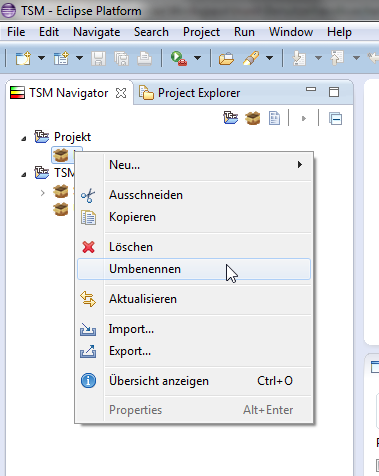
\includegraphics[width= 260px]{BilderHandbuchTSMNavigator/Paket/PaketUmbenennen.png}
\caption{Paket Umbenennen}
\label{fig:PaketUmbenennen}
\end{figure}

\item Geben Sie nun den neuen Namen Ihres Pakets an. Bitte beachten Sie, dass die folgenden Zeichen nicht erlaubt sind: $ < > ? " : | _ . \setminus / *$
\end{enumerate}


\subsection{Testfall}
Ein Testfall ist eine Folge von Testschritten, die der Tester umsetzt. Er kann Teil eines Pakets oder eines Projekts sein.
\subsubsection{Testfall anlegen}

\begin{enumerate}
\item Selektieren Sie das Projekt oder Paket in dem der Testfall erstellt werden soll. Klicken Sie anschließend oben im TSM-Navigator auf das Testfall-Symbol.

\begin{figure}[H]
\centering
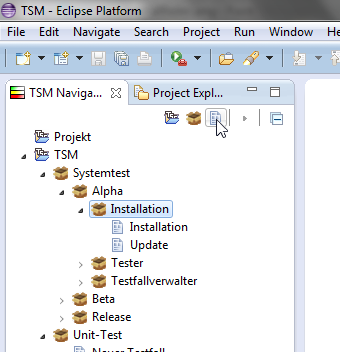
\includegraphics[width= 240px]{BilderHandbuchTSMNavigator/Testfall/Testfall.png}
\caption{Testfall anlegen}
\label{fig:Testfall}
\end{figure}

\item Ein neuer Registerreiter öffnet sich, in dem die Daten des Testfalls eingegeben werden können.

\begin{figure}[H]
\centering
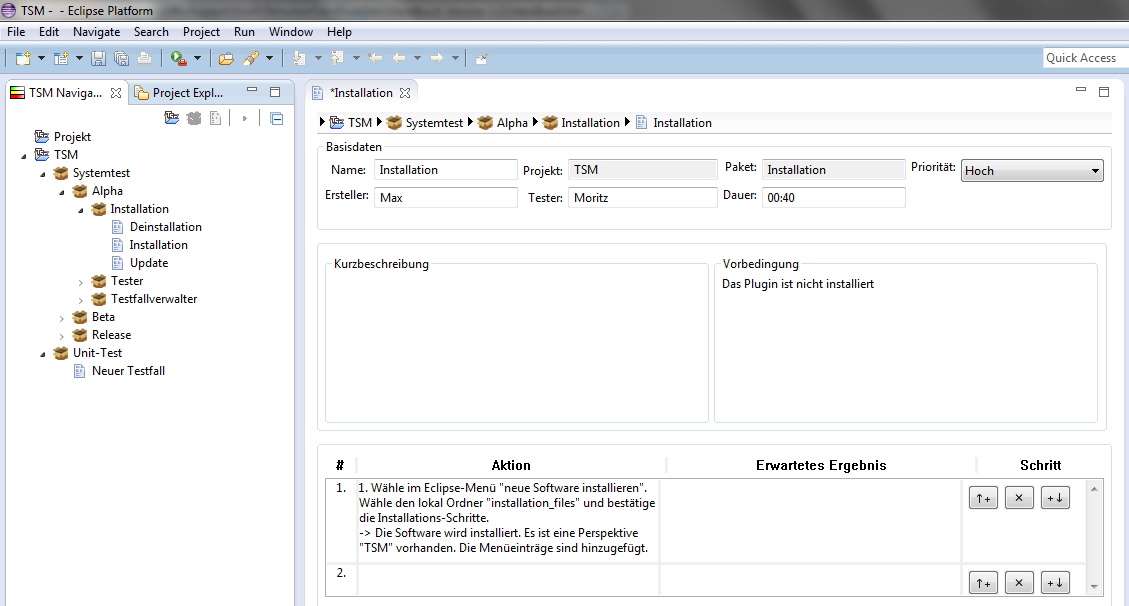
\includegraphics[width= 350px]{BilderHandbuchTSMNavigator/Testfall/TestfallReiter.png}
\caption{Testfall}
\label{fig:TestfallReiter}
\end{figure}

\item Speichern Sie, indem Sie oben in der Menüleiste auf das
Diskettensymbol klicken

\includegraphics[width= 15px]{BilderHandbuch/Testfall/Disk.png}
\\ oder per Tastenkombination \texttt{STRG+S}.

\end{enumerate}
\textit{\textbf{Alternativ} können Sie auch per Rechtsklick im TSM-Navigator unter \texttt{New...} - \texttt{TSM-Testfall} einen Testfall anlegen.
Oder per Tastenkombination \texttt{STRG+N} öffnet sich ein Assistent, indem Sie unter dem Ordner \texttt{TSM} auf \texttt{TSM-Testfall} klicken und dem Assistenten folgen.}

\subsubsection{Testfall umbenennen}
\begin{enumerate}
\item Machen Sie einen Rechtsklick auf den Testfall, den Sie umbenennen möchten und klicken Sie auf \texttt{Umbenennen}.

\begin{figure}[H]
\centering
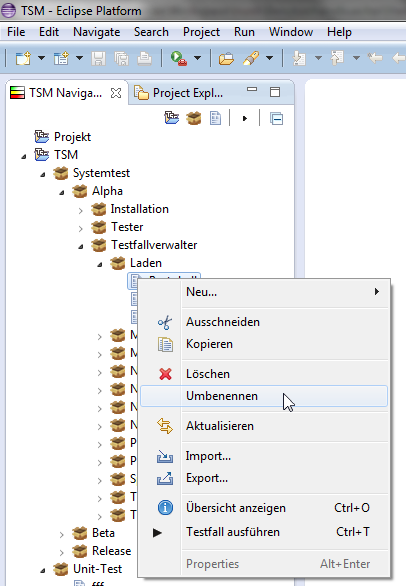
\includegraphics[width= 260px]{BilderHandbuchTSMNavigator/Testfall/TestfallUmbenennen.png}
\caption{Testfall Umbenennen}
\label{fig:TestfallUmbenennen}
\end{figure}

\item Geben Sie nun den neuen Namen Ihres Testfalls an. Bitte beachten Sie, dass die folgenden Zeichen nicht erlaubt sind: $ < > ? " : | _ . \setminus / *$
\end{enumerate}

\textit{\textbf{Alternativ} können Sie auch einen Doppelklick auf den Testfall machen und ihn dann im Bearbeitungsmodus umbenennen.}

\subsubsection{Testfall bearbeiten}
\begin{enumerate}
\item Machen Sie ein Doppelklick auf den Testfall, welchen Sie bearbeiten möchten.
\item Ein neuer Registerreiter öffnet sich mit den Daten des Testfalls. Sie können nun alles bearbeiten.
\item Speichern Sie, indem Sie oben in der Menüleiste auf das
Diskettensymbol klicken

\includegraphics[width= 15px]{BilderHandbuch/Testfall/Disk.png}
\\ oder per Tastenkombination \texttt{STRG+S}.
\end{enumerate}

\subsubsection{Formatierung im Editor}
Richttextfelder bezeichnen die Felder im Testfall die editierbar und formatierbar sind, wie die \texttt{Kurzbeschreibung}, die \texttt{Vorbedingung} oder 
in den Testschritten \texttt{Aktion} und \texttt{Erwartetes Ergebnis}.
\paragraph{Formatierung}
\begin{enumerate}
\item Markieren Sie das Wort oder den Text welchen Sie editieren möchten und machen Sie einen Rechtsklick darauf.

\begin{figure}[H]
\centering
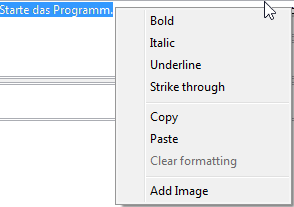
\includegraphics[width= 160px]{BilderHandbuch/Testfall/Formatieren.png}
\caption{Formatieren mit Rechtsklick}
\label{fig:AddImage}
\end{figure}

\item Wählen Sie eine dieser Formatierungen aus und klicken Sie darauf:\\
\texttt{Fett}, \texttt{Kursiv}, \texttt{Unterstrichen}, \texttt{Durchstreichen}.
\end{enumerate}
Möchten Sie die gesamte Formatierung aufheben, so markieren Sie das Wort oder den Text und wählen Sie per Rechtsklick \texttt{Formatierung aufheben}.\\
Zusätzlich gibt es noch die zwei Funktionen \texttt{Kopieren} und \texttt{Einfügen} um Text zu kopieren und einzufügen. 

\paragraph{Bild einfügen}
\begin{enumerate}

\begin{figure}[H]
\centering
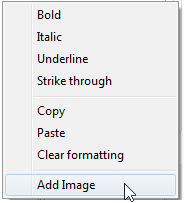
\includegraphics[width= 100px]{BilderHandbuch/Testfall/AddImage.png}
\caption{Bild einfügen mit Rechtsklick}
\label{fig:AddImage}
\end{figure}

\item Machen Sie einen Rechtsklick im Editor an der gewünschten Stelle und wählen Sie \texttt{Bild einfügen} aus, es erscheint ein Dateiauswahldialog.
\item Suchen Sie nach Ihrem gewünschten Bild und klicken Sie auf \texttt{Öffnen}.
\item Das Bild erscheint nun klein in einer neuen Zeile.
\end{enumerate}

Die Bilder im Editor können skaliert werden.
Dazu können Sie entweder auf das Symbol in der oberen rechten Bildecke klicken um es auf Maximalgröße zu skalieren oder am Symbol in der unteren rechten Ecke ziehen, um es zu skalieren.
Des Weiteren öffnet sich ein Vorschaufenster, wenn Sie auf das Bild klicken.
Im Vorschaufenster können Sie die Bildansicht mit Hilfe des Mausrads vergrößern oder verkleinern und mittels Zug mit dem Mauszeiger verschieben.

\subsubsection{Testfall ausführen}
\begin{enumerate}
\item Selektieren Sie den Testfall, welchen Sie ausführen möchten und klicken Sie oben im TSM-Navigator auf das Startsymbol.

\includegraphics[width= 15px]{BilderHandbuchTSMNavigator/Testfall/Play.png}.
\item Ihr Testfall öffnet sich als neuer Registerreiter.

Wenn Sie den Mauszeiger über das blaue Informationssymbol halten, können Sie die Kurzbeschreibung sehen.
Darunter ist die Vorbedingung und in der Tabelle werden die einzelnen Testschritte nochmals angezeigt.


\begin{figure}[H]
\centering
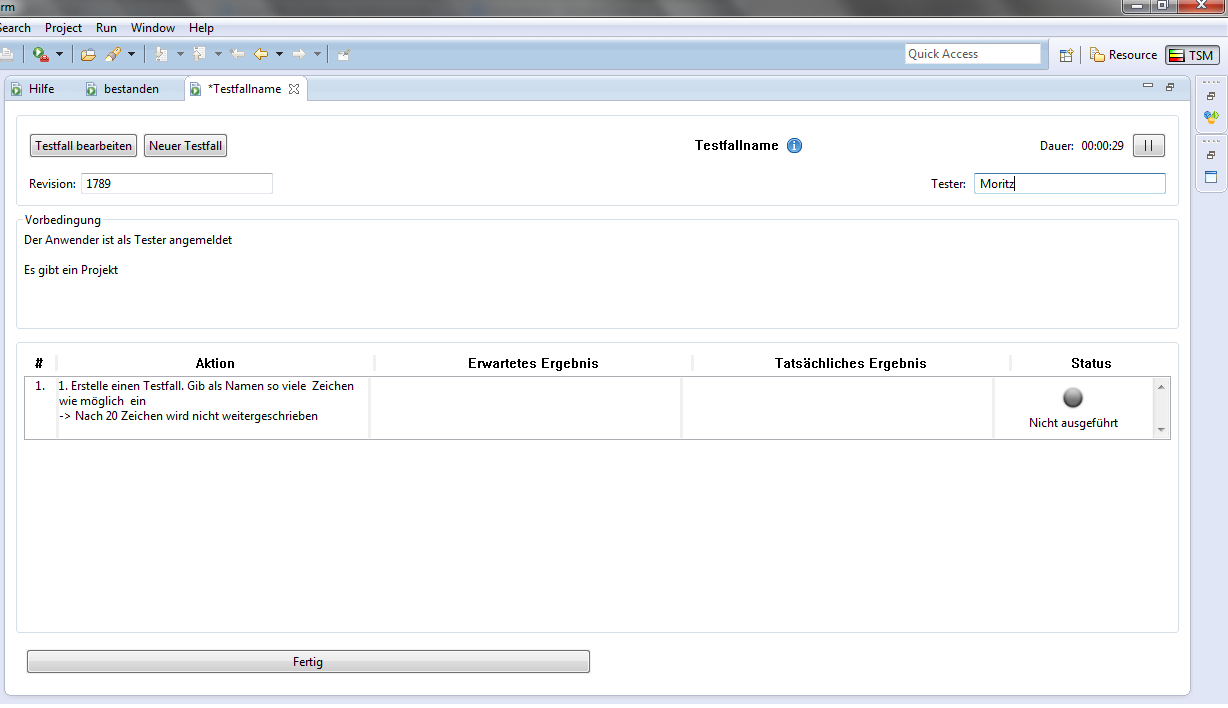
\includegraphics[width= 470px]{BilderHandbuch/Testfall/Ausfuehren.png}
\caption{Ein Testfall wird gerade ausgeführt}
\label{fig:Ausfuehren}
\end{figure}

In der Spalte \texttt{Status} gibt es einen Kreis.
Dieser ist anfangs grau (\texttt{nicht ausgeführt}), was bedeutet, dass der Schritt noch nicht durchgeführt wurde. Durch anklicken wird er erst grün (\texttt{bestanden}), 
dann gelb (\texttt{bestanden mit Anmerkungen}) und dann rot (\texttt{nicht bestanden}), beim nächsten Klick steht er wieder auf \texttt{nicht ausgeführt}.

Sollten Fehler in der Testfallbeschreibung gefunden werden, kann über die \texttt{Testfall bearbeiten}-Schaltfläche in die Testfall-bearbeiten-Ansicht gewechselt werden. \\
Oben rechts befindet sich eine Stoppuhr, sie startet sobald man den Test ausführt.
Man kann die Stoppuhr auch pausieren lassen. Sie setzt sich jedes Mal zurück, sobald man einen neuen Testfall ausführt.

\item Nachdem der Testfall durchgeführt wurde, kann das Endresultat beschrieben werden indem man auf \texttt{Fertig} klickt.
\item Der Wert in der Auswahlbox wird automatisch auf die höchste verwendete Fehlerfarbe gesetzt, kann aber noch geändert werden.
\item Schreiben Sie Ihr Endresultat und klicken Sie auf \texttt{Speichern} oder \texttt{Abbrechen}.
\end{enumerate}
Sobald Sie das Endresultat speichern, öffnet sich das Protokoll des Testfalls.\\
\\\
Sollten Sie bei der Ausführung einmal die falsche Revision eingegeben haben, können Sie diese in der .xml-Datei ändern.
Öffnen Sie hierzu das Protokoll mit dem xml-Editor im Project Explorer. Ändern Sie den Punkt \texttt{Revision} und speichern Sie.

\subsection{Protokoll anzeigen}
Sobald Sie das Endresultat gespeichert haben, erscheint eine Protokolldatei unter dem Testfall, den Sie gerade ausgeführt haben.
\begin{enumerate}
\item Klicken Sie zweimal auf das gewünschte Protokoll.

\begin{figure}[H]
\centering
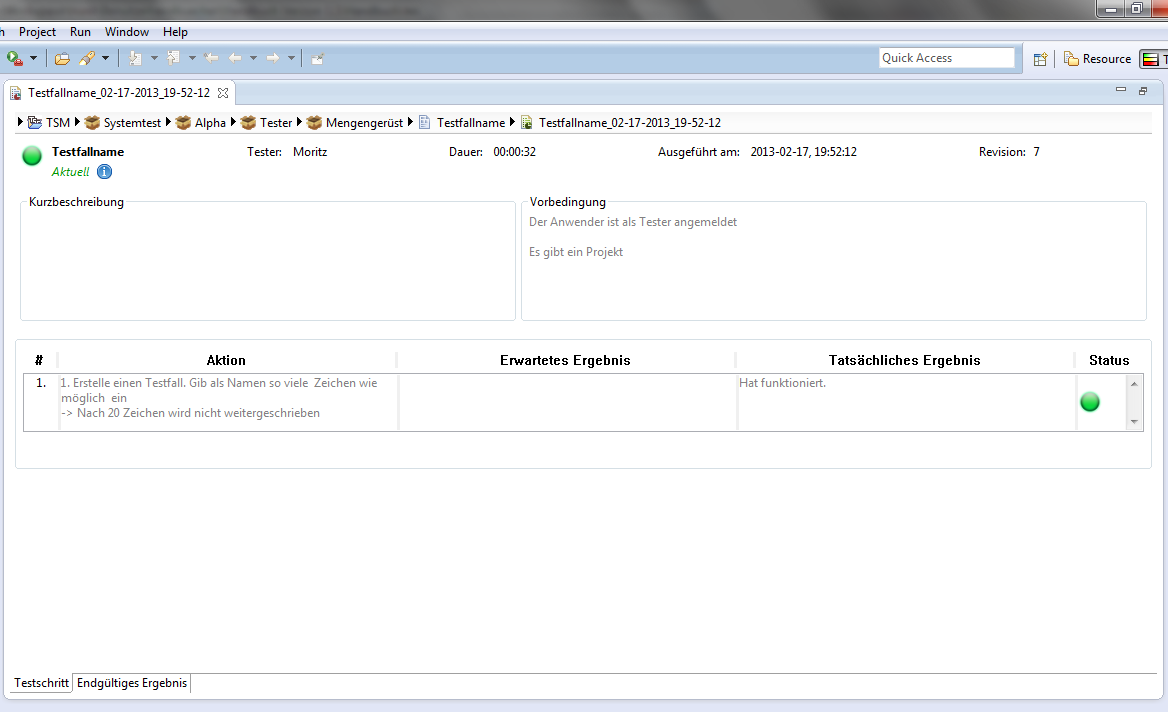
\includegraphics[width= 320px]{BilderHandbuch/Protokoll/Protokoll.png}
\caption{Endresultat beschreiben}
\label{fig:Protokoll}
\end{figure}

\item Es öffnet sich ein neuer Registerreiter, in dem die Daten und Ergebnisse des Testfalls zu sehen sind.
\item Wenn Sie unten auf den Registerreiter \texttt{Endgültiges Ergebnis} klicken, so sehen Sie das Endresultat.
\end{enumerate}


\begin{figure}[H]
\centering
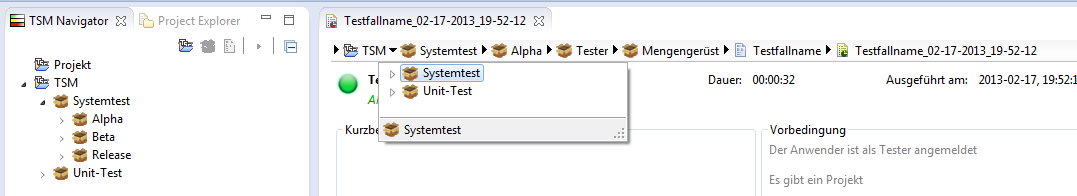
\includegraphics[width= 260px]{BilderHandbuch/Protokoll/Breadcrumb.png}
\caption{So können Sie ein anderes Protokoll auswählen}
\label{fig:Breadcrumb}
\end{figure}

Oben in der Breadcrumb-Leiste können Sie zwischen den einzelnen Projekten/Paketen/Testfällen umschalten um andere Protokolle oder Testfälle anzeigen lassen.

\subsection{TSM-Schnellansicht}
Auf der rechten Seite finden Sie die \texttt{TSM-Schnellansicht}.
Falls nicht, so klicken Sie in der Menüleiste auf \texttt{Fenster} -- \texttt{Zeige Ansicht} -- \texttt{Andere...} -- Und dann im TSM-Ordner auf Schnellansicht.

\begin{figure}[H]
\centering
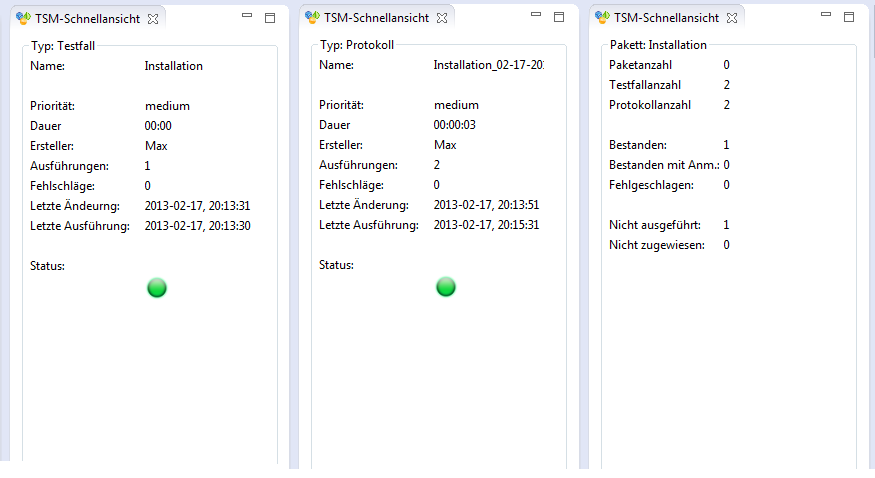
\includegraphics[width= 320px]{BilderHandbuch/Quickview/Quickview.png}
\caption{Verschiedene Ansichten}
\label{fig:Breadcrumb}
\end{figure}

Die Schnellansicht zeigt den Status des jeweiligen selektierten Objekts an.\\
Rechts sehen Sie die Schnellansicht eines beispielhaften Projekts, in der Mitte ein Paket und links sehen Sie die eines Testfalls.

\newpage
\subsection{PDF-Export}
Protokolle wie auch Testfälle können als PDF-Datei exportiert werden.
\begin{enumerate}

\item Machen Sie einen Rechtsklick im TSM-Navigator und wählen Sie \texttt{Export...} aus.

\begin{figure}[H]
\centering
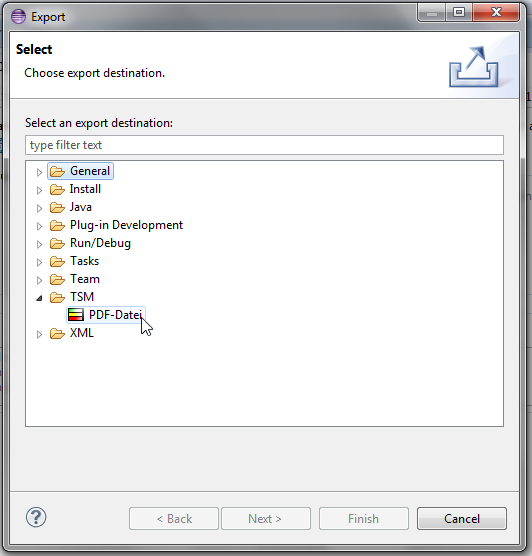
\includegraphics[width= 260px]{BilderHandbuch/PDF/ExportA.png}
\caption{PDF-Export öffnen}
\label{fig:ExportA}
\end{figure}

\item Wählen Sie im Assistenten \texttt{TSM} und dann \texttt{PDF-Datei} aus und klicken Sie auf \texttt{Next}.
\item Es öffnet sich ein Assistent, in dem Sie alle Testfälle oder Protokolle auswählen können, welche Sie exportieren möchten.

\begin{figure}[H]
\centering
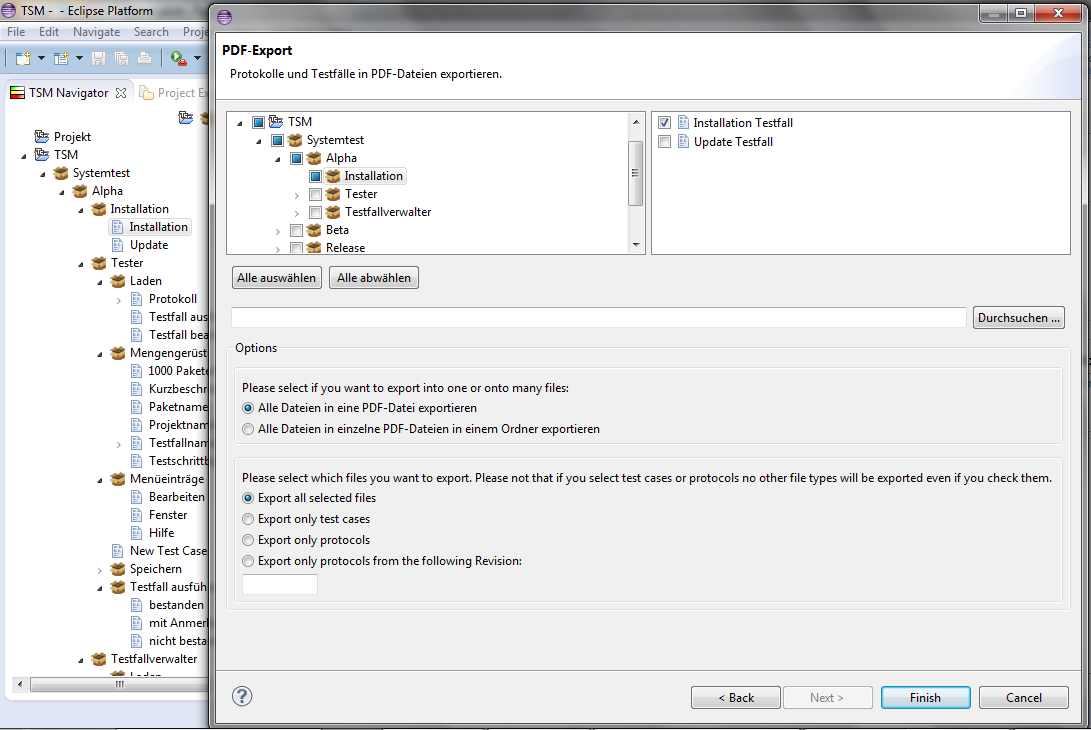
\includegraphics[width= 300px]{BilderHandbuch/PDF/ExportB.png}
\caption{Pakete und Testfälle als PDF-Datei exportieren}
\label{fig:ExportB}
\end{figure}

\item Wählen Sie ein Verzeichnis aus, in das exportiert werden soll, indem Sie auf \texttt{Durchsuchen...} klicken
\item Sie können entweder alle selektierten Testfälle in ein großes PDF-Dokument exportieren oder in einzelne Dokumente. Dabei wird dann die Ordnerstruktur aus Eclipse übernommen.\\
Des Weiteren könne Sie wahlweise nur Testfälle, nur Protokolle oder nur Protokolle einer bestimmten Revision exportieren. 
\item Klicken Sie nun auf \texttt{Finish}.
\item Die PDF-Dateien liegen nun in dem Verzeichnis, welches Sie zuvor ausgewählt haben.
\end{enumerate}

\subsection{Justus-Import}
Es gibt die Möglichkeit, Dateien des Systemtestwerkzeuges Justus (\url{http://justus.tigris.org/}) zu importieren. Bitte beachten Sie, dass für den Import bereits ein Projekt angelegt sein muss. 
\begin{enumerate}
\item Machen Sie einen Rechtsklick im TSM-Navigator und wählen Sie \texttt{Import...} aus.
\item Wählen Sie im Assistenten \texttt{TSM} \texttt{Justus-Datei} aus und klicken Sie auf \texttt{Next}.
\item Es öffnet sich ein Assistent, in dem Sie eine Datei zum Importieren auswählen können. 
\item Wählen Sie ein Verzeichnis aus, in dem Sie auf \texttt{Durchsuchen...} klicken
\item Wählen Sie ein Zielprojekt oder einen Zielordner aus.
\item Sie können entweder eine Justus-Testschritt als einen TSM-Testschritt importieren oder eine Justus-Sequenz als einen TSM-Testschritt. 
\item Klicken Sie nun auf \texttt{Finish}.
\item In dem gewählten Ordner befinden sich nun die importierten Testfälle. 
\end{enumerate}

\subsection{Übersicht}
Sie zeigt Ihnen eine Übersicht der einzelnen Revisionen der verschiedenen Protokolle an, um den Status von ganzen Projekten, Paketen oder Testfällen zu erhalten.
Sie zeigt Ihnen zu jedem Testfall und zu jedem ausgewählten Revision jeweils das neueste zugehörige Protokoll an.
Sie können die gewollten Revisionen oben durch Klick auf \texttt{Auswählen} aussuchen die angezeigt werden sollen.
Zur Übersicht kommen Sie, wenn Sie einen Rechtsklick auf einen Testfall/Paket oder Projekt machen und auf \texttt{Übersicht anzeigen} klicken.\\
Die Zahl in Klammern sind dabei die Anzahl an Testfällen, die zu dieser Revision ein Protokoll haben.
Sollte die Übersicht trotz einer vorhandenen Selektion nichts anzeigen, so selektieren Sie etwas anderes und dann erneut Ihre gewünschte Selektion.


\subsection{TSM-Filteransicht}
Unten finden Sie die Filterung (\texttt{TSM-Filteransicht}).
Falls nicht, so klicken Sie auf der Menüleiste auf \texttt{Fenster} -- \texttt{Zeige Ansicht} -- \texttt{Andere...} -- und klicken anschließend im TSM-Ordner auf Filteransicht.

In der Filterung kann man nach Testfällen oder nach Protokollen filtern.
Um beispielsweise nach einem Testfall zu filtern, der am 30.01.2012 von Max erstellt wurde und dessen Priorität auf "`Hoch"' gesetzt ist, würde die Filterung so aussehen:

\begin{figure}[H]
\centering
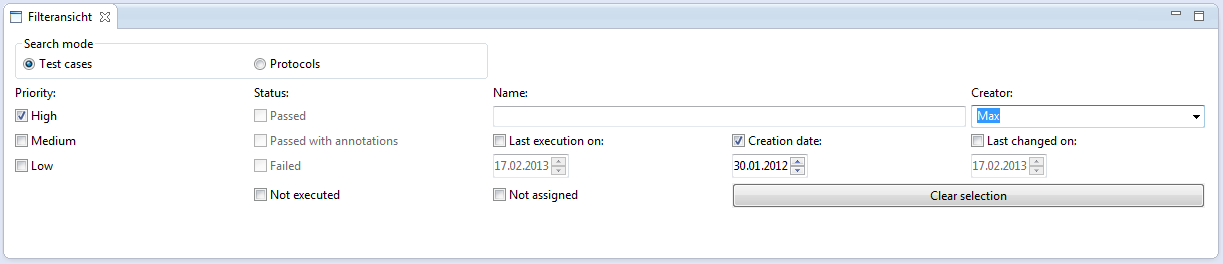
\includegraphics[width= 320px]{BilderHandbuch/Filterung/FilterungA.png}
\caption{Beispiel: Filterung}
\label{fig:FilterungA}
\end{figure}

Filtert man nach einem Protokoll das Moritz am 17.02.2012 getestet hat und den Namen weiß, so filtert man so danach:

\begin{figure}[H]
\centering
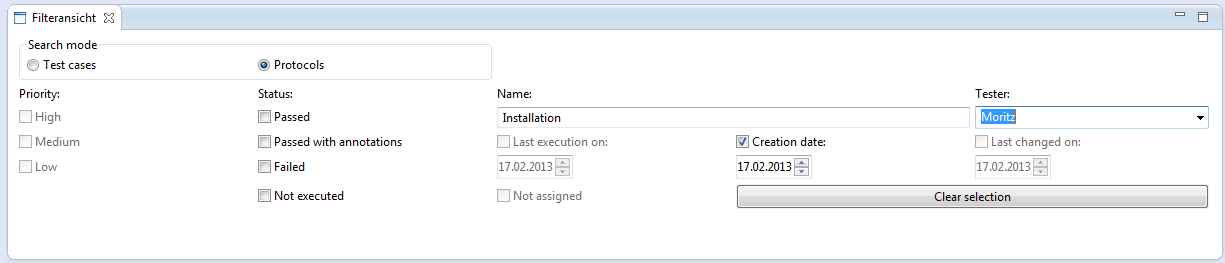
\includegraphics[width= 320px]{BilderHandbuch/Filterung/FilterungB.png}
\caption{Beispiel: Filterung}
\label{fig:FilterungB}
\end{figure}

Die Ergebnisse der Filterung erscheint links im TSM-Navigator, es werden nur die Testfälle/Protokolle angezeigt nach denen man Filtert.

Klickt man auf \texttt{Clear selection}, so wird alles aufgehoben und alle Protokolle und Testfälle erscheinen im TSM-Navigator wieder.

\textbf{Achtung, im Project Explorer kann man nicht filtern!}

\newpage
\section{Benutzung im Project Explorer}
\subsection{Projekt}
Ein Projekt ist der Überbegriff für eine Sammlung von Paketen und Testfällen.

\subsubsection{Projekt anlegen: }
\begin{enumerate}
\begin{figure}[H]
\centering
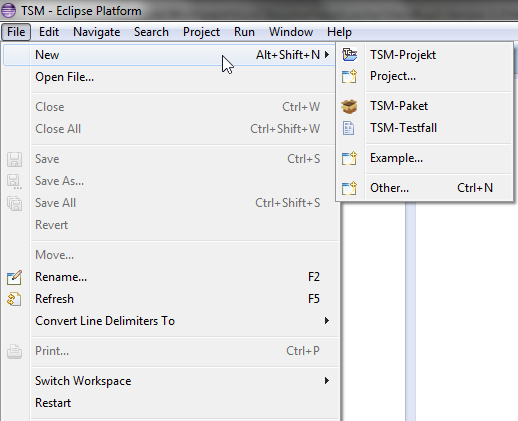
\includegraphics[width= 260px]{BilderHandbuch/AnlegenM.png}
\caption{Projekt über die Menüleiste anlegen}
\label{fig:AnlegenM}

\end{figure}

\item Klicken Sie auf \texttt{Datei} in der Menüleiste und halten Sie den Mauszeiger über \texttt{Neu}.
\item Im erscheinenden Menü klicken Sie auf \texttt{TSM-Projekt}, es öffnet sich ein Assistent.

\begin{figure}[H]
\centering
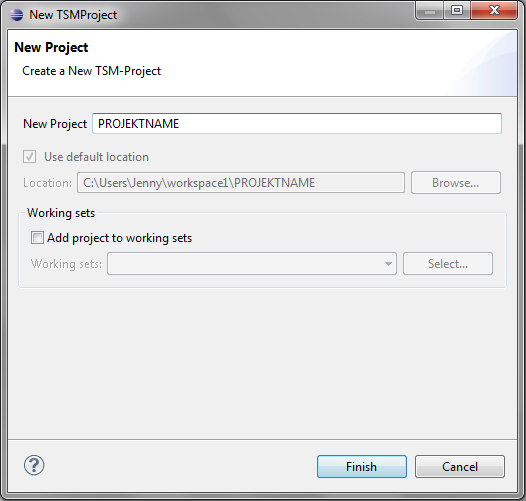
\includegraphics[width= 260px]{BilderHandbuch/Projekt/NewProject.png}
\caption{Projekt anlegen}
\label{fig:NewProject}
\end{figure}

\item Im Assistenten geben Sie in \texttt{Neues Projekt} den Namen Ihres Projekts an und klicken auf \texttt{Finish}. Das Projekt liegt nun im Project Explorer.
\end{enumerate}

\textit{\textbf{Alternativ} können Sie auch per Rechtsklick im TSM-Navigator unter \texttt{New...} - \texttt{TSM-Projekt} ein Projekt anlegen.
Oder Sie öffnen per Tastenkombination \texttt{STRG+N} den Assistenten. Wählen Sie dort \texttt{TSM} und dann \texttt{TSM-Projekt} folgen Sie dem Assistenten.}


\subsubsection{Projekt umbenennen}
\begin{enumerate}
\item Machen Sie einen Rechtsklick auf das Projekt, das Sie umbenennen möchten.


\begin{figure}[H]
\centering
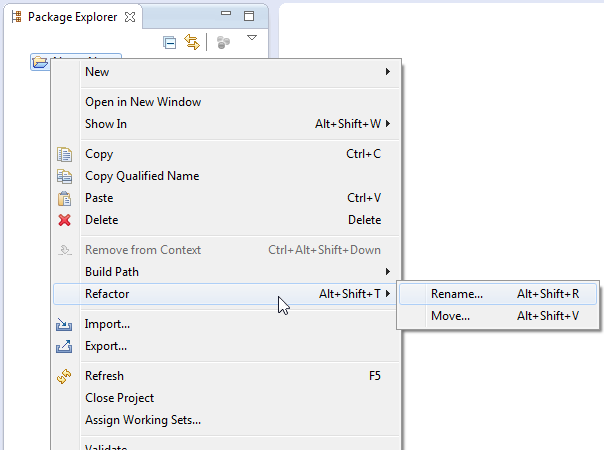
\includegraphics[width= 260px]{BilderHandbuch/UmbenennenR.png}
\caption{Wählen Sie \texttt{Refactor} und dann \texttt{Rename...} im Kontexmenü}
\label{fig:UmbennenR1}
\end{figure}

\item Wählen Sie \texttt{Refactor}, dann \texttt{Rename...}.

\begin{figure}[H]
\centering
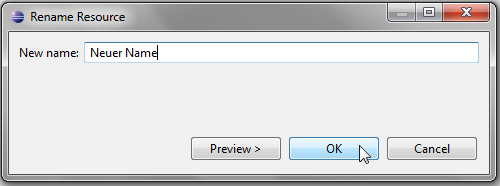
\includegraphics[width= 200px]{BilderHandbuch/UmbenennenFenster.png}
\caption{Geben Sie einen neuen Namen ein}
\label{fig:UmbenennenFenster2}
\end{figure}

\item Geben Sie im Fenster den neuen Namen Ihres Projekts an und klicken Sie auf \texttt{Ok}. Das Projekt wird umbenannt.
Bitte beachten Sie, dass die folgenden Zeichen nicht erlaubt sind: $ < > ? " : | _ . \setminus / *$
\end{enumerate}

\subsection{Paket}
Ein Paket ist eine Struktureinheit, um ein Projekt logisch untergliedern zu können. Pakete können Testfälle und weitere Pakete enthalten.

\subsubsection{Paket anlegen}
Um ein Paket anlegen zu können muss bereits ein Projekt angelegt sein.
\begin{enumerate}
\begin{figure}[H]
\centering
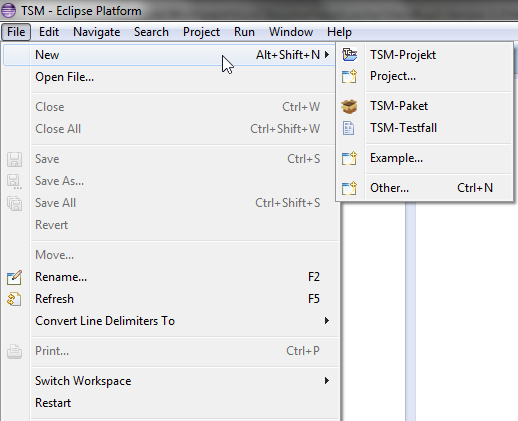
\includegraphics[width= 260px]{BilderHandbuch/AnlegenM.png}
\caption{Paket über die Menüleiste anlegen}
\label{fig:AnlegenM2}
\end{figure}

\item Klicken Sie auf \texttt{Datei} in der Menüleiste und halten Sie den Mauszeiger über \texttt{Neu}.
\item Im erscheinenden Menü klicken Sie auf \texttt{TSM Package}, es öffnet sich ein Assistent.

\begin{figure}[H]
\centering
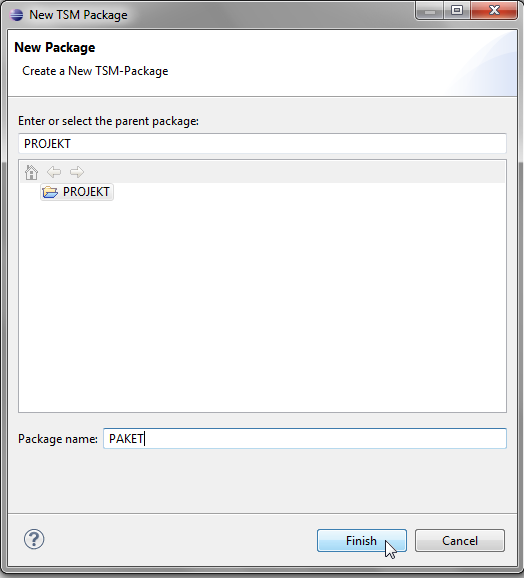
\includegraphics[width= 260px]{BilderHandbuch/Paket/NewPackage.png}
\caption{Paket anlegen}
\label{fig:NewPackage}
\end{figure}

\item Geben Sie im Assistenten den Namen Ihres Pakets an und klicken Sie auf \texttt{Finish}. Das Paket liegt nun im Project Explorer.
\end{enumerate}

\textit{\textbf{Alternativ} können Sie auch per Rechtsklick im TSM-Navigator unter \texttt{New...} - \texttt{TSM-Paket} ein Paket anlegen.
Oder per Tastenkombination \texttt{STRG+N} öffnet sich ein Assistent indem Sie unter dem Ordner \texttt{TSM} auf \texttt{TSM-Paket} klicken und dem Assistenten folgen.}

\subsubsection{Paket umbenennen}
\begin{enumerate}
\item Machen Sie einen Rechtsklick auf das Paket, das Sie umbenennen möchten.

\begin{figure}[H]
\centering
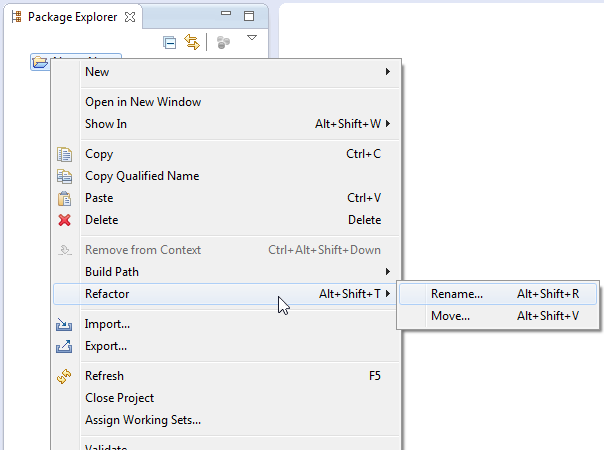
\includegraphics[width= 260px]{BilderHandbuch/UmbenennenR.png}
\caption{Wählen Sie \texttt{Refactor} und dann \texttt{Rename...} im Kontextmenü}
\label{fig:UmbenennenR}
\end{figure}

\item Wählen Sie \texttt{Refactor}, dann \texttt{Rename...}.

\begin{figure}[H]
\centering
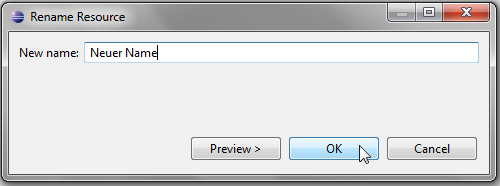
\includegraphics[width= 200px]{BilderHandbuch/UmbenennenFenster.png}
\caption{Geben Sie einen neuen Namen ein}
\label{fig:UmbenennenFenster}
\end{figure}

\item Geben Sie im Fenster den neuen Namen Ihres Pakets an und klicken Sie auf \texttt{Ok}. Das Paket wird umbenannt.
Bitte beachten Sie, dass die folgenden Zeichen nicht erlaubt sind:$ < > ? " : | _ . \setminus / *$
\end{enumerate}

\subsection{Testfall}
Ein Testfall ist eine Folge von Testschritten, die der Tester umsetzt. Er kann Teil eines Pakets oder eines Projekts sein.

\subsubsection{Testfall anlegen}
Um einen neuen Testfall anzulegen, wird ein Paket oder Projekt selektiert.
Falls Sie das falsche Projekt/Paket selektiert haben, können Sie im Assistenten auf \texttt{Durchsuchen...} klicken und das Projekt/Paket selektieren, in dem der Testfall erstellt werden soll.

\begin{figure}[H]
\centering
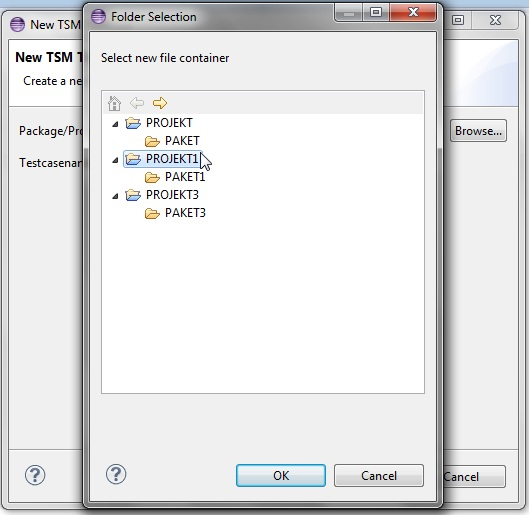
\includegraphics[width= 260px]{BilderHandbuch/Testfall/Browse.png}
\caption{Selektieren Sie das Projekt oder Paket in dem der Testfall erstellt werden soll}
\label{fig:Browse}
\end{figure}

\begin{enumerate}
\item Klicken Sie auf \texttt{Datei} in der Menüleiste und halten Sie den Mauszeiger über \texttt{Neu}.

\begin{figure}[H]
\centering
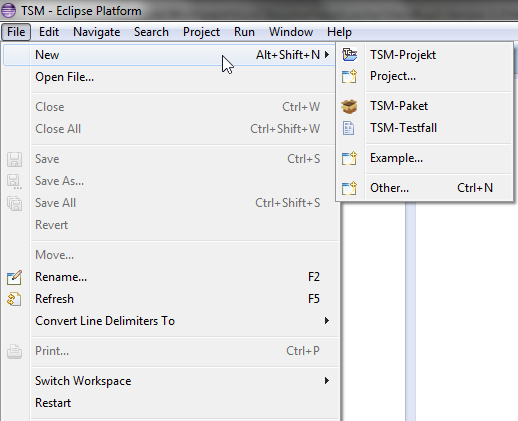
\includegraphics[width= 260px]{BilderHandbuch/AnlegenM.png}
\caption{Testfall über die Menüleiste anlegen}
\label{fig:AnlegenM}
\end{figure}

\item Im erscheinenden Kontextmenü klicken Sie auf \texttt{TSM Testcase}, es öffnet sich ein Assistent.

\begin{figure}[H]
\centering
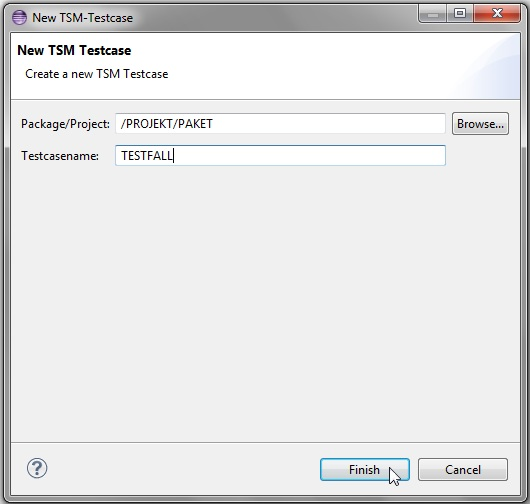
\includegraphics[width= 260px]{BilderHandbuch/Testfall/NewTestcase.png}
\caption{Testfall anlegen}
\label{fig:NewTestcase}
\end{figure}

\item Geben Sie im Assistenten den Namen Ihres Testfalls an und klicken Sie auf \texttt{Fertig}.\\
Falls Sie das falsche Projekt/Paket selektiert haben, können Sie im Assistenten auf \texttt{Durchsuchen...} klicken. Sehen Sie dazu die Abbildung \ref{fig:Browse}.
\item Ein neuer Registerreiter öffnet sich, in dem die Daten des Testfalls eingegeben werden können.
\item Speichern Sie, indem Sie oben in der Menüleiste auf das
Diskettensymbol klicken

\includegraphics[width= 15px]{BilderHandbuch/Testfall/Disk.png}
\\ oder per Tastenkombination \texttt{STRG+S}.

\end{enumerate}

\textit{\textbf{Alternativ} können Sie auch per Rechtsklick im TSM-Navigator unter \texttt{New...} - \texttt{TSM-Testfall} einen Testfall anlegen.
Oder per Tastenkombination \texttt{STRG+N} öffnet sich ein Assistent, indem Sie unter dem Ordner \texttt{TSM} auf \texttt{TSM-Testfall} klicken und dem Assistenten folgen.}
\subsubsection{Testfall umbenennen}
\begin{enumerate}
\item Machen Sie einen Rechtsklick auf den Testfall, welchen Sie umbenennen möchten.

\begin{figure}[H]
\centering
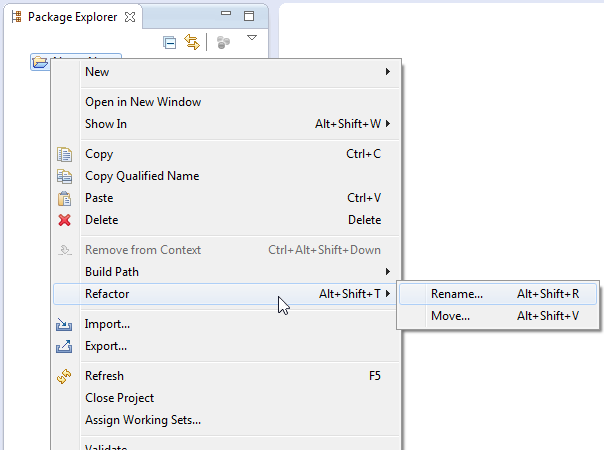
\includegraphics[width= 260px]{BilderHandbuch/UmbenennenR.png}
\caption{Wählen Sie \texttt{Refactor} und dann \texttt{Rename...} im Kontextmenü}
\label{fig:UmbenennenR}
\end{figure}

\item Wählen Sie \texttt{Refactor}, dann \texttt{Rename...}.

\begin{figure}[H]
\centering
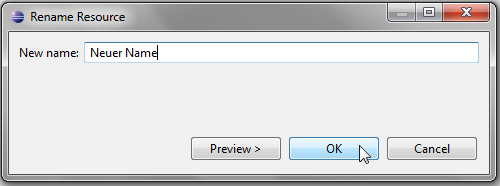
\includegraphics[width= 200px]{BilderHandbuch/UmbenennenFenster.png}
\caption{Geben Sie einen neuen Namen ein}
\label{fig:UmbenennenFenster}
\end{figure}

\item Geben Sie im Fenster den neuen Namen Ihres Testfalls an und klicken Sie auf \texttt{Ok}. Der Testfall wird umbenannt.
Bitte beachten Sie, dass die folgenden Zeichen nicht erlaubt sind: $ < > ? " : | _ . \setminus / *$
\end{enumerate}

\textit{\textbf{Alternativ} können Sie auch einen Doppelklick auf den Testfall machen und ihn dann im Bearbeitungsmodus umbenennen.}

\subsubsection{Testfall bearbeiten}
\textbf{Achtung}, es öffnet sich immer der letzte benutzte Editor. Wählen Sie gegebenenfalls über das Kontextmenü \texttt{Öffnen mit} und dann \texttt{Test Case Editor}.
\begin{enumerate}
\item Machen Sie ein Doppelklick auf den Testfall, welchen Sie bearbeiten möchten.
\item Ein neuer Registerreiter öffnet sich mit den Daten des Testfalls. Sie können nun alles bearbeiten.
\item Speichern Sie, indem Sie oben in der Menüleiste auf das
Diskettensymbol klicken

\includegraphics[width= 15px]{BilderHandbuch/Testfall/Disk.png}
\\ oder per Tastenkombination \texttt{STRG+S}.
\end{enumerate}

\subsubsection{Formatierung im Editor}
Richtexteditoren bezeichnen die Felder im Testfall die editierbar und
formatierbar sind, wie z.\,B.: \texttt{Kurzbeschreibung}, \texttt{Vorbedingung} in den Testschritten \texttt{Aktion} und \texttt{Erwartetes Ergebnis}.
\paragraph{Formatierung}
\begin{enumerate}
\item Markieren Sie das Wort oder den Text welchen Sie editieren möchten und machen Sie einen Rechtsklick darauf.

\begin{figure}[H]
\centering
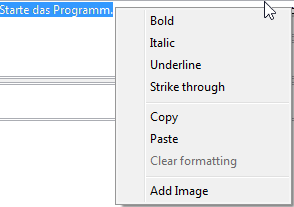
\includegraphics[width= 160px]{BilderHandbuch/Testfall/Formatieren.png}
\caption{Formatieren mit Rechtsklick}
\label{fig:AddImage}
\end{figure}

\item Wählen Sie einer dieser Formatierungen aus und klicken Sie darauf:\\
\textbf{fett}, \texttt{kursiv}, \uline{unterstrichen} , \sout{durchgestrichen}.
\end{enumerate}
Möchten Sie die Formatierung aufheben, so markieren Sie das Wort oder den Text und wählen Sie per Rechtsklick \texttt{Formatierung aufheben}.\\
\texttt{Kopieren} und \texttt{Einfügen} steht für Kopieren und Einfügen.

\paragraph{Bild einfügen}
\begin{enumerate}

\begin{figure}[H]
\centering
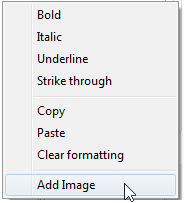
\includegraphics[width= 100px]{BilderHandbuch/Testfall/AddImage.png}
\caption{Bild einfügen mit Rechtsklick}
\label{fig:AddImage}
\end{figure}


\item Machen Sie einen Rechtsklick im Editor an der gewünschten Stelle und wählen Sie \texttt{Bild hinzufügen} aus, es erscheint ein Dateiauswahldialog.
\item Suchen Sie nach Ihrem gewünschten Bild und klicken Sie auf \texttt{Öffnen}.
\item Das Bild erscheint nun klein in einer neuen Zeile.
\end{enumerate}

\subsubsection{Testfall ausführen}
\begin{enumerate}
\item Selektieren Sie den Testfall, welchen Sie ausführen möchten.

\begin{figure}[H]
\centering
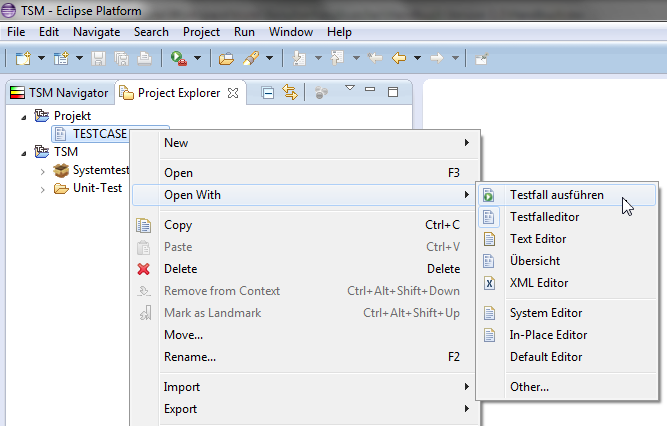
\includegraphics[width= 320px]{BilderHandbuch/Testfall/OpenWith2.png}
\caption{Wählen Sie \texttt{Öffnen mit} und dann \texttt{Execute Test} im Kontextmenü}
\label{fig:OpenWith2}
\end{figure}

\item Machen Sie einen Rechtsklick und wählen Sie \texttt{Öffnen mit} und dann \texttt{Execute Test} aus.
\item Im Reiter öffnet sich Ihr Testfall.
Wenn Sie den Mauszeiger über das blaue Informationssymbol halten, so können Sie die Kurzbeschreibung sehen.
\\
Darunter ist die Vorbedingung und in der Tabelle werden die einzelnen Testschritte nochmals angezeigt.

\begin{figure}[H]
\centering
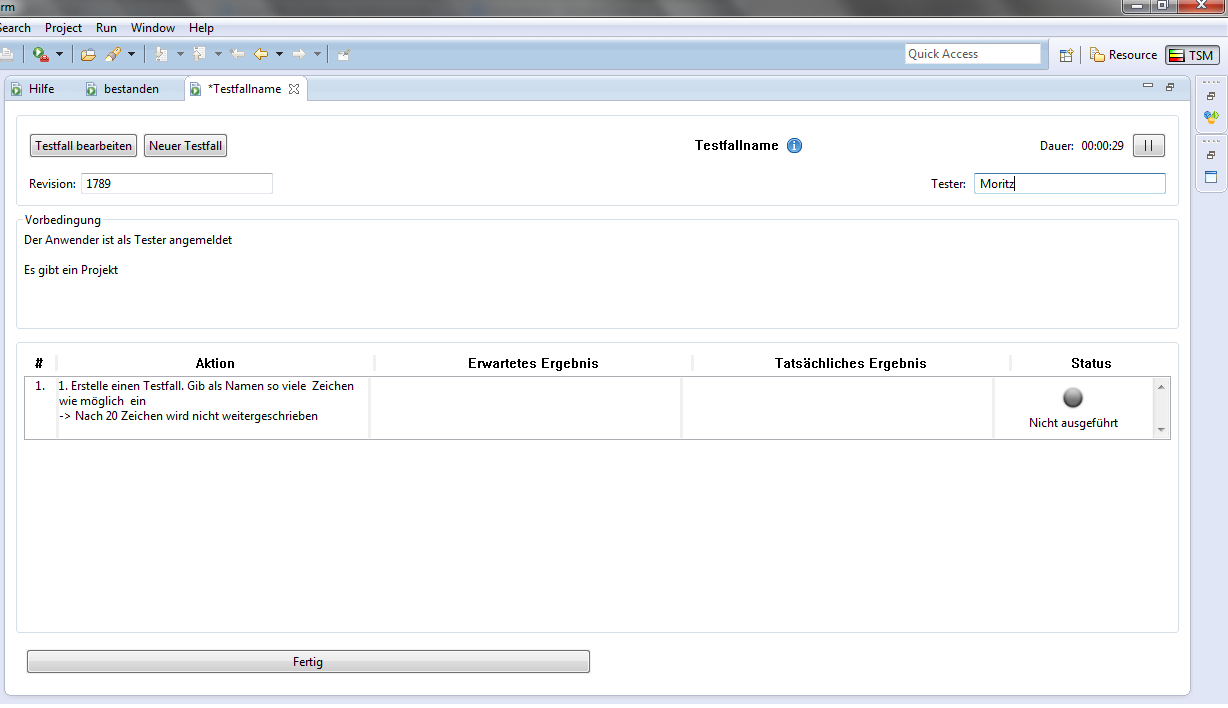
\includegraphics[width= 380px]{BilderHandbuch/Testfall/Ausfuehren.png}
\caption{Testfall ausführen}
\label{fig:Ausfuehren}
\end{figure}

\item In der Spalte \texttt{Tatsächliches Ergebnis} wird das aktuelle Resultat des Testschrittes eingegeben.
In der Spalte \texttt{Status} gibt es einen Kreis.
Dieser ist anfangs grau (\texttt{nicht ausgeführt}), was bedeutet, dass der Schritt noch nicht durchgeführt wurde. Durch anklicken wird er erst grün (\texttt{bestanden}), 
dann gelb (\texttt{bestanden mit Anmerkungen}) und dann rot (\texttt{nicht bestanden}), beim nächsten Klick steht er wieder auf \texttt{nicht ausgeführt}.

Sollten Fehler in der Testfallbeschreibung gefunden werden, kann über die \texttt{Testfall bearbeiten}-Schaltfläche in die Testfall-bearbeiten-Ansicht gewechselt werden.
Oben links befindet sich eine Stoppuhr, sie startet sobald man den Test ausführt. Man kann die Stoppuhr auch pausieren lassen.
Sie setzt sich jedes Mal zurück, sobald man einen neuen Testfall ausführt. 

\item Nachdem der Testfall durchgeführt wurde, kann das Endresultat beschrieben werden indem man auf \texttt{Fertig} klickt.
\item Der Wert in der Auswahlbox wird automatisch auf die höchste verwendete Fehlerfarbe gesetzt, kann aber noch geändert werden.
\item Schreiben Sie Ihr Endresultat und klicken Sie auf \texttt{Speichern} oder \texttt{Abbrechen}.
\end{enumerate}
Sobald Sie das Endresultat speichern, öffnet sich das Protokoll des Testfalls.\\
\\\
Sollten Sie bei der Ausführung einmal die falsche Revision eingegeben haben. können Sie diese in der .xml-Datei ändern.
Öffnen Sie hierzu das Protokoll mit dem xml-Editor. Ändern Sie den Punkt \texttt{Revision} und speichern Sie. 

\subsection{Protokoll anzeigen}
Sobald Sie das Endresultat gespeichert haben, erscheint eine Protokolldatei über dem Testfall, den Sie gerade ausgeführt haben.
\begin{enumerate}
\item Klicken Sie zweimal auf das gewünschte Protokoll.

\begin{figure}[H]
\centering
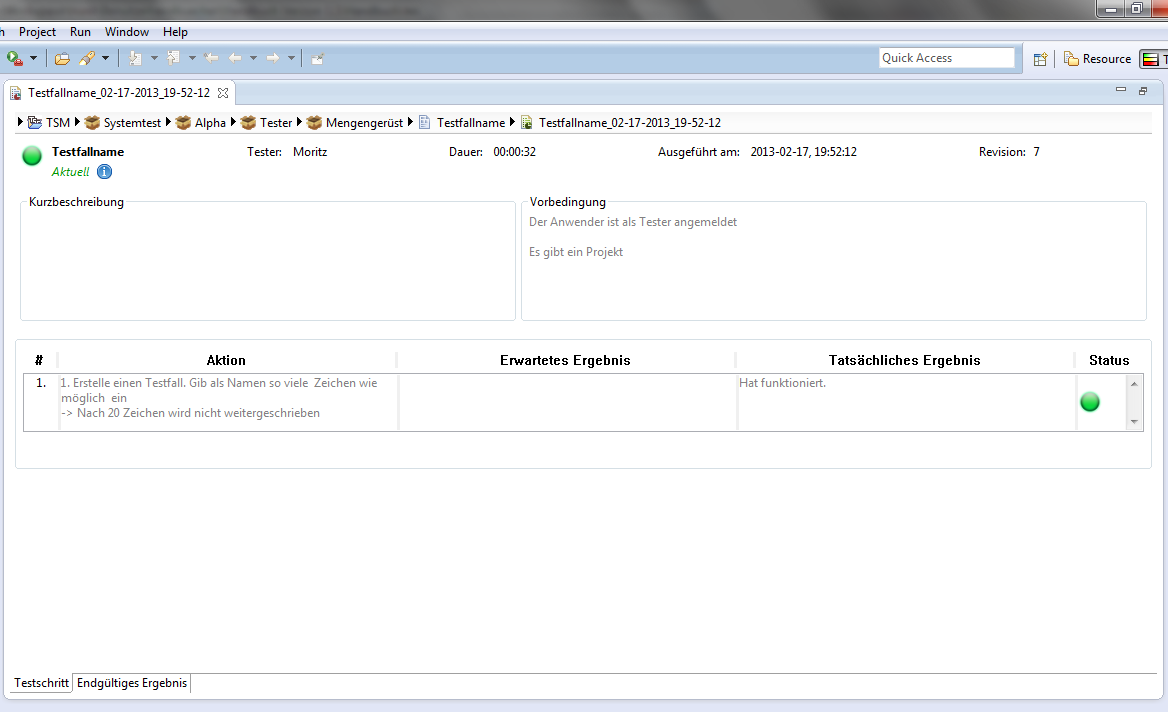
\includegraphics[width= 320px]{BilderHandbuch/Protokoll/Protokoll.png}
\caption{Endresultat beschreiben}
\label{fig:Protokoll}
\end{figure}

\item Es öffnet sich ein neuer Registerreiter, in dem die Daten und Ergebnisse des Testfalls zu sehen sind.
\item Wenn Sie unten auf den Registerreiter \texttt{Endgültiges Ergebnis} klicken, so sehen Sie das Endresultat.
\end{enumerate}


\begin{figure}[H]
\centering
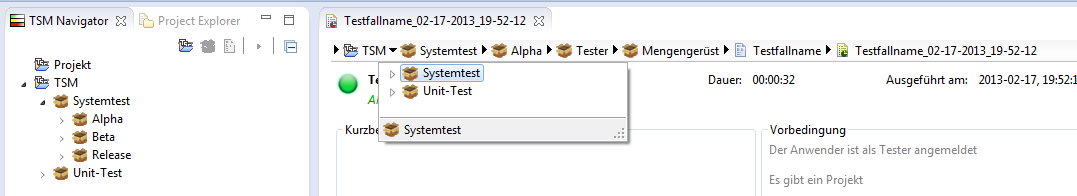
\includegraphics[width= 360px]{BilderHandbuch/Protokoll/Breadcrumb.png}
\caption{So können Sie ein anderes Protokoll auswählen}
\label{fig:Breadcrumb}
\end{figure}

Oben in der Breadcumb-Leiste können Sie zwischen den einzelnen Projekten/Paketen/Testfällen umschalten um andere Protokolle anzeigen zu lassen.

\subsection{TSM-Schnellansicht}
Auf der rechten Seite finden Sie die \texttt{TSM-Schnellansicht}.

\begin{figure}[H]
\centering
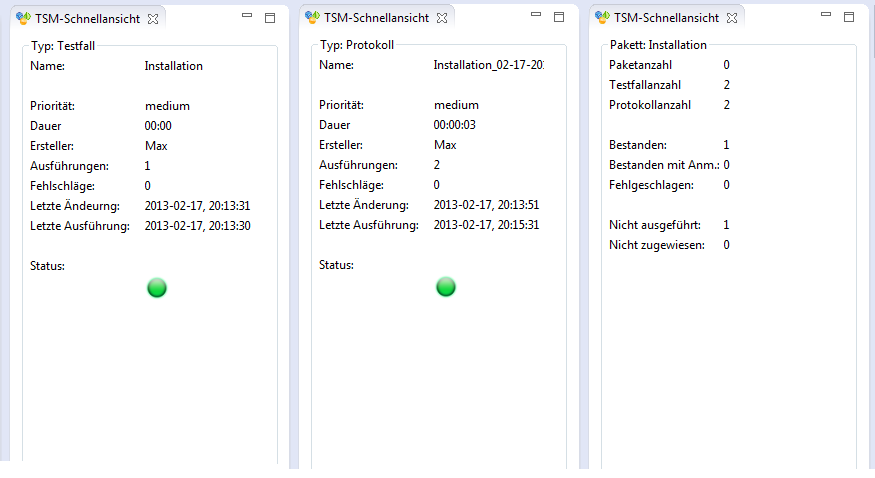
\includegraphics[width= 320px]{BilderHandbuch/Quickview/Quickview.png}
\caption{Verschiedene Ansichten}
\label{fig:Quickview}
\end{figure}

Die Schnellansicht zeigt den Status des jeweiligen selektierten Objekts an.\\
In Abbildung \ref{fig:Quickview} sehen Sie links die Schnellansicht eines beispielhaften Testfall, in der Mitte ein beispielhaftes Protokoll und rechts ein beispielhaftes Paket.

\newpage
\subsection{PDF-Export}
Protokolle wie auch Testfälle können als PDF-Datei exportiert werden.
\begin{enumerate}
\begin{figure}[H]
\centering
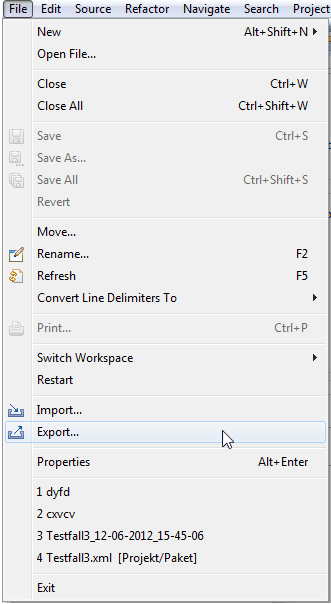
\includegraphics[width= 120px]{BilderHandbuch/PDF/Export.png}
\caption{Datei als PDF-Datei exportieren}
\label{fig:Export}
\end{figure}

\item Klicken Sie oben in der Menüleiste auf \texttt{File} dann \texttt{Export...}.

\begin{figure}[H]
\centering
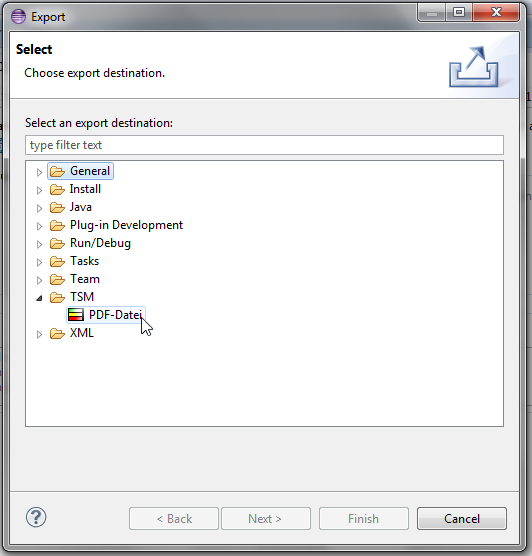
\includegraphics[width= 260px]{BilderHandbuch/PDF/ExportA.png}
\caption{PDF-Export öffnen}
\label{fig:ExportA}
\end{figure}

\item Wählen Sie im Assistenten \texttt{TSM} und dann \texttt{PDF-Datei} aus und klicken Sie auf \texttt{Weiter}.
\item Es öffnet sich ein Assistent, in dem Sie alle Testfälle oder Protokolle auswählen können, welche Sie exportieren möchten.

\begin{figure}[H]
\centering
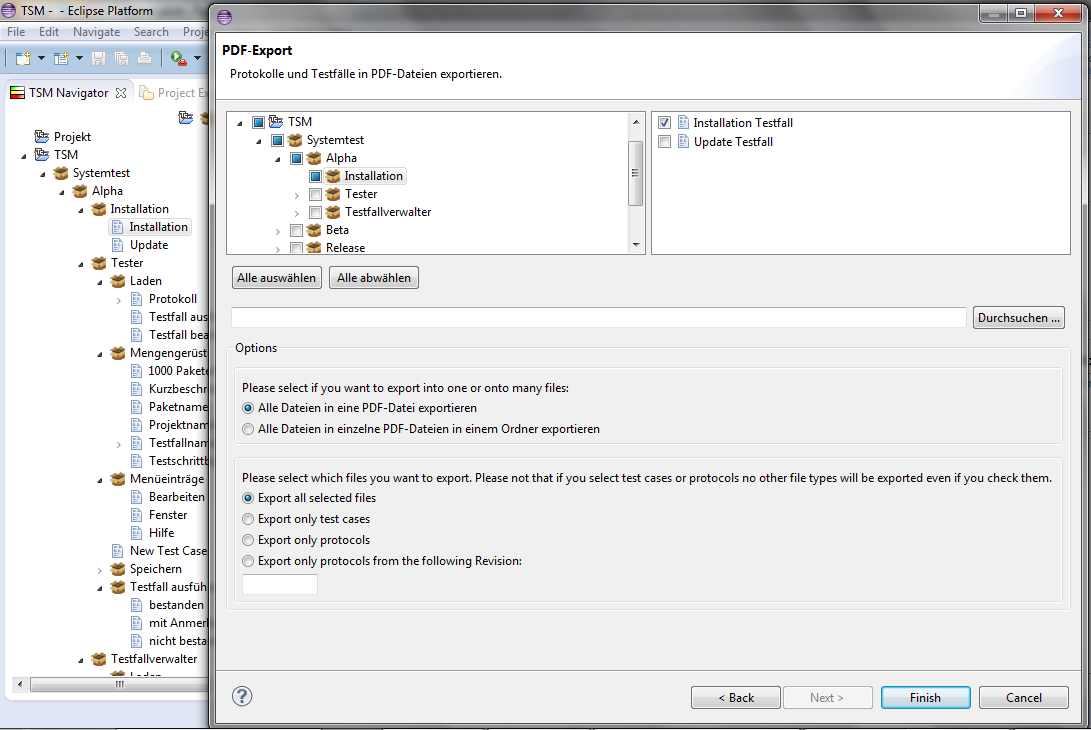
\includegraphics[width= 360px]{BilderHandbuch/PDF/ExportB.png}
\caption{Datei als PDF-Datei exportieren}
\label{fig:ExportB}
\end{figure}

\item Wählen Sie ein Verzeichnis aus, in dem Sie auf \texttt{Durchsuchen...} und dann auf \texttt{Fertig} klicken.
\item Die PDF-Dateien liegen nun in dem Verzeichnis, welches Sie zuvor ausgewählt haben.
\end{enumerate}

\subsection{Justus-Import}
Es gibt die Möglichkeit, Dateien des Systemtestwerkzeuges Justus (\url{http://justus.tigris.org/}) zu importieren. Bitte beachten Sie, dass für den Import bereits ein Projekt angelegt sein muss. 
\begin{enumerate}
\item Machen Sie einen Rechtsklick im TSM-Navigator und wählen Sie \texttt{Import...} aus.
\item Wählen Sie im Assistenten \texttt{TSM} \texttt{Justus-Datei} aus und klicken Sie auf \texttt{Next}.
\item Es öffnet sich ein Assistent, in dem Sie eine Datei zum Importieren auswählen können. 
\item Wählen Sie ein Verzeichnis aus, in dem Sie auf \texttt{Durchsuchen...} klicken
\item Wählen Sie ein Zielprojekt oder einen Zielordner aus.
\item Sie können entweder eine Justus-Testschritt als einen TSM-Testschritt importieren oder eine Justus-Sequenz als einen TSM-Testschritt. 
\item Klicken Sie nun auf \texttt{Finish}.
\item In dem gewählten Ordner befinden sich nun die importierten Testfälle. 
\end{enumerate}

\subsection{Übersicht}
Sie zeigt Ihnen eine Übersicht der einzelnen Revisionen der verschiedenen Protokolle an, um den Status von ganzen Projekten, Paketen oder Testfällen zu erhalten.
Sie zeigt Ihnen zu jedem Testfall und zu jedem ausgewählten Revision jeweils das neueste zugehörige Protokoll an.
Sie können die gewollten Revisionen oben durch Klick auf \texttt{Auswählen} aussuchen die angezeigt werden sollen.
Zur Übersicht kommen Sie, wenn Sie einen Rechtsklick auf einen Testfall/Paket oder Projekt machen und auf \texttt{Übersicht anzeigen} klicken.\\
Die Zahl in Klammern sind dabei die Anzahl an Testfällen, die zu dieser Revision ein Protokoll haben.
Sollte die Übersicht trotz einer vorhandenen Selektion nichts anzeigen, so selektieren Sie etwas anderes und dann erneut Ihre gewünschte Selektion.


\section{Bekannte Probleme}
Die Probleme sind von schwerwiegend nach unproblematisch sortiert.\\

\subsection*{Testfälle dürfen nicht in nicht-TSM-Projekte verschoben werden}
Momentan können Testfälle nicht in nicht-TSM-Projekten erstellt werden. Das Verschieben dorthin ist allerdings möglich.
Dort kann jedoch nicht für einen reibungslosen Ablauf aller Funktionalitäten garantiert werden.

\subsection*{Per \textit{refactor} $ \rightarrow $ \textit{rename} kann ein Name mit mehr als 200 Zeichen eingegeben werden}
Per \textit{refactor} $ \rightarrow $ \textit{rename} kann ein Name mit mehr als 200 Zeichen eingegeben werden. 
Auch wird dort nicht auf die unter Windows im Dateinamen verbotenen Zeichen überprüft.
Dies geschieht erst, nachdem der Testfall erneut zum Bearbeiten geöffnet wurde. Daher wird empfohlen auf die gewählten Zeichen und die Länge der Namen zu achten.

\subsection*{Unklares Verhalten bei Auschneiden/Kopieren und Einfügen von Bildern}
In einigen Fällen wird beim Kopieren und Wiedereinfügen von Bildern der Text in Form von HTML eingefügt.

\subsection*{Einfügen von Bildern einer vorherigen Sitzung funktioniert nicht}
Bilder, die kopiert wurden und nach einem anschließenden Neustarten der Software wieder eingefügt werden resultieren in einem nicht-druckbaren Zeichen und werden nicht angezeigt.

\subsection*{Scrollen mit Mausrad in der Übersicht geht nicht}
Manuell ist es relativ langsam. Außerdem kann man nicht nach rechts scrollen wenn zu viele Revisionen angezeigt werden.

\subsection*{Tastenkürzel unter Linux bei der RCP-Version}
Bei manchen Systemkonfigurationen werden Tastenkürzel ohne aktiviert, ohne dass die Strg-Taste gedrückt wurde oder gedrückt gehalten wird.
Dies hat zur Folge dass z.\,B. ein bloßes Drücken von "`N"' den Assistenten öffnet.

\subsection*{Kaufmannsund in Dateinamen nicht möglich}
Bilder, deren Dateiname oder Pfad ein Kaufmannsund (\&) enthält können nicht eingefügt und angezeigt werden.

\subsection*{Projekte können im TSM-Navigator nicht ausgeschnitten oder kopiert und eingefügt werden}
Um dieses Problem zu umgehen sollte ein neues TSM-Projekt angelegt werden und anschließend der gesamte Inhalt kopiert werden.
Man sollte dabei beachten, dass Protokolle nicht mit kopiert werden können. Diese können nur verschoben werden.

\subsection*{Verwaiste Protokolle werden in der Übersicht nicht berücksichtigt}
Löscht man einen Testfall aber nicht seine zugehörigen Protokolle, so bleiben diese ohne zugehörigen Testfall. Sie werden dann in der Übersicht nicht mehr berücksichtigt.

\subsection*{Die Übersicht kann in bestimmten Fällen nicht geöffnet werden}
Sind bereits andere Testfälle oder Protokolle offen, so kann es vorkommen dass die Übersicht sich nicht anzeigen lässt (ohne Hinweis oder Meldung).
Um das Problem zu beheben sollten alle offenen Testfälle oder Protokolle geschlossen werden.

\subsection*{Unklare Fehlermeldung beim Export von nicht vorhandener Revision}
Exportiert man eine Revision die nicht vorhanden ist, erscheint eine unklare Fehlermeldung: "`Sie haben keine Datei zum Exportieren ausgewählt."'

\subsection*{Beim Export-Abbruch wird eine PDF-Datei erstellt}
Der Abbruch-Button beim Export ist ohne Funktion, die PDF-Datei wird trotzdem erstellt.

\subsection*{Felder mit Informationen in oberer Leiste werden teilweise im Protokoll abgeschnitten}
Im Protokoll werden Informationen in oberer Leiste werden teilweise abgeschnitten.

\subsection*{Formatierung wird auch nach Leerzeichen beibehalten}
Markiert man ein Wort oder ein Satz im Richttextfeld und wählt \texttt{Formatierung aufheben} und macht gleich danach einen Leerzeichen und schreibt weiter, wird die Formatierung beibehalten.
Erst ein Zeilenumbruch hebt die Formatierung ohne Zuhilfenahme des Kontextmenüs auf.

\subsection*{Gleichzeitiges Öffnen eines Testfalls zum Bearbeiten, Ausführen und in der Übersicht führt zu keiner Fehlermeldung}
Testfall ausführen dominiert in diesem Falle. Übersicht öffnen kann man am Anfang und später Testfall bearbeiten oder ausführen.

\subsection*{Einige Tastenkürzel fehlen im TSM-Navigator}
Der TSM-Navigator kann nicht alle Tastenkürzel die im Project Explorer vorhanden sind.

\subsection*{Quickview: Name des Testfalls skaliert nicht mit Fensterbreite}
Ist der Name eines Projekts/Pakets oder Testfall zu lang wird er nicht vollständig in der Schnellansicht angezeigt.

\subsection*{About-Dialog: Feld "`Provider"' ist leer}
Geht man über \texttt{Help} - \texttt{About Eclipse Platform} in TSM hinein, so ist das Feld Provider noch leer.

\subsection*{Ein Bild im Vorschaufenster verschieben}
Möchte man das Bild im Vorschaufenster verschieben, so kann das Bild in manchen Fällen verschmieren.

\subsection*{Beim Ausführen einen neuen Testfall anlegen}
Möchte man beim Ausführen einen neuen Testfall erstellen so ist der Assistent nicht mit sinnvollen Standardwerten ausgefüllt.

\subsection*{Kontextmenü zeigt aktivierte Formatierung nicht an}
Markiert man im Richttextfeld ein Wort oder einen Satz und formatiert diesen anschließend und öffnet es erneut, ist diese Formatierung im Kontextmenü nicht sichtbar.

\subsection*{Bilder in Protokoll werden nicht ganz dargestellt}
In einigen Fällen werden die Bilder im Protokoll nicht ganz dargestellt.

\subsection*{Unter Windows XP werden Texte unter der Breadcrumb in der Protokollansicht abgeschnitten}
Unter dem Betriebssystem Windows XP können längere Bezeichnungen unter der Breadcrumb im Protokoll abgeschnitten werden.

\subsection*{Flackern des Mauszeigers beim Skalieren von Bildern}
In manchen Fällen flackert der Mauszeiger beim Skalieren von Bildern oder verschwindet.

\subsection*{Richtext: Großer "`Eingabestrich"' flackert über Bilder drüber}
In einigen Fällen flackert ein Strich über den Richttextbildern nach dem ein Bild skaliert wurde.

\subsection*{Sekunden von "`Letzte Änderung"' werden in Schnellansicht abgeschnitten}
In manchen Systemkonfigurationen wird die letzte Sekunde der Zeitangabe "`Letzte Änderung"' in der Schnellansicht nicht angezeigt.

\subsection*{Sehr kleine Bilder werden nicht gezeichnet}
Ist das Bild zu klein wird ein Obj-Symbol gezeichnet.


\section{Versionsgeschichte}

\subsection*{0.1 -- 15.02.2013}
\begin{itemize}
 \item Erste Fassung.
\end{itemize}

\subsection*{0.2 -- 17.02.2013}
\begin{itemize}
 \item Aktualisiert
 \item Kapitel TSM-Navigator hinzugefügt
 \item Kapitel Filterung hinzugefügt
\end{itemize}
 
\subsection*{0.3 -- 18.02.2013}
\begin{itemize}
 \item Rechtschreibfehler korrigiert.
 \item Bug liste aktualisiert.
 \item Installation aktualisiert.
 \item Kapitel Overview hinzugefügt.
\end{itemize}

\subsection*{0.4 -- 24.09.2014}
\begin{itemize}
 \item Anpassung an Version 1.5.1.
 \item Rechtschreibfehler korrigiert und aufgeräumt.
\end{itemize}

\subsection*{0.5 -- 20.11.2014}
\begin{itemize}
 \item Anpassung an Version 1.5.2.
\end{itemize}

 
\end{document}

